\newacronym{tclab}{TCLab}{\textit{Temperature Control Lab}}

\chapter{Planta piloto}
\label{ch:planta_piloto}

O sistema experimental usado para o projeto de ações de controle é uma mini planta piloto chamada \acrlong{tclab}
(do inglês, Laboratório de Controle de Temperatura), ou apenas \acrshort{tclab}\footnote{                       % footnote
    Maiores informações sobre o \acrshort{tclab} podem ser encontrados em \href{http://apmonitor.com/heat.htm}{http://apmonitor.com/heat.htm}.
}. Esta planta foi desenvolvida na \textit{Brigham Young University} (BYU) e apresentada pela primeira vez no
\textit{2017 ASEE Summer School}, na \textit{North Carolina State University} (NCSU). Foi desenvolvida com o
propósito de facilitar o acesso de estudantes a um laboratório de testes de controle.

Esta mini planta é essencialmente um \textit{shield} para Arduino\footnote{
    Arduino é uma plataforma de prototipagem eletrônica de hardware livre e de placa única, projetada com um    % footnote
    microcontrolador Atmel AVR com suporte de entrada/saída embutido.                                           % footnote
} contendo 2 aquecedores e 2 sensores de temperatura, mostrado na \cref{fig:tclab}. A energia dos aquecedores é
transferida através de condução, convecção e radiação até os sensores de temperatura. Tanto o controle da
potência dos aquecedores quanto as medições realizadas pelos sensores são efetuados através do Arduino.

O \acrshort{tclab} possibilita fazer a programação do controle da mini planta utilizando linguagem Python,
\acrshort{matlab} ou Simulink.

\begin{figure}[h]
	\caption{Laboratório de Controle de Temperatura}
	\begin{center}
		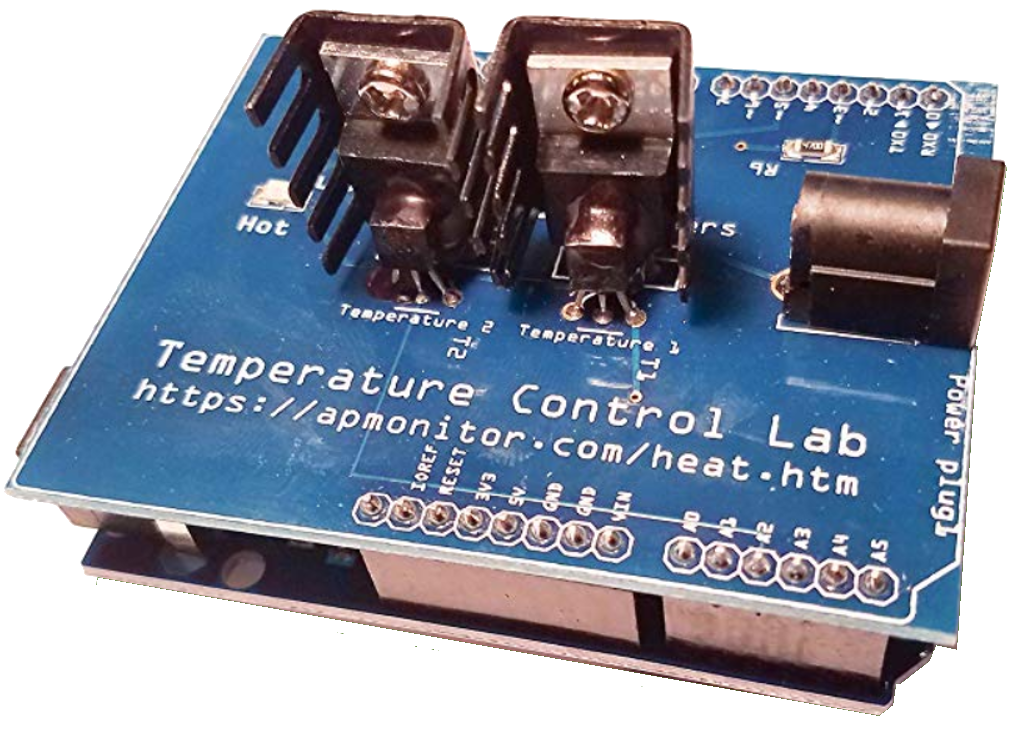
\includegraphics[width=0.55\textwidth]{./5_images/tclab.png} 
		\label{fig:tclab}
	\end{center}
	\centering
	\makebox[\width]{Fonte: ?????}  % TODO Corrigir autor
\end{figure}

% =====================================================================================================
% ============================================= Section ===============================================
% =====================================================================================================
\section{Modelagem da planta piloto}
\label{sec:modelagem_da_planta_piloto}

% TODO Adicionar modelagem descrita no http://apmonitor.com/pdc/index.php/Main/ArduinoModeling e nos Labs A e B